\documentclass[border=0.2cm]{standalone}
\usepackage{tikz}
\begin{document}
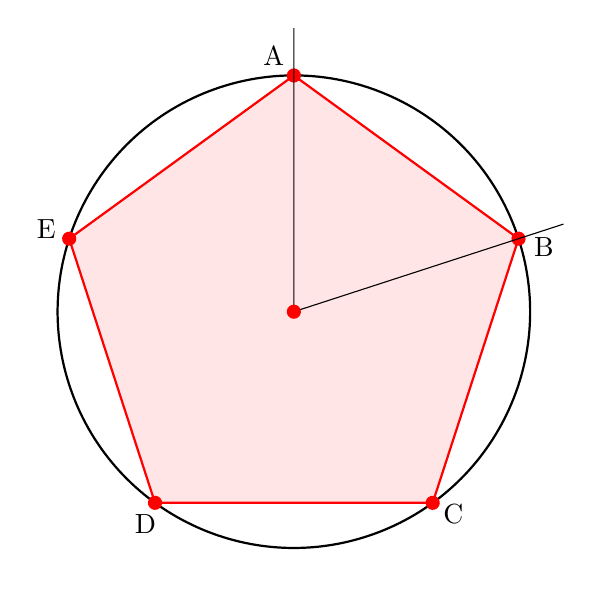
\begin{tikzpicture}[scale=3,rotate=18]
    \draw[thick] (0,0) circle (1cm);
    \draw[thick,red,fill=red!10] (0:1) -- (72:1) -- (2*72:1) -- (3*72:1) -- (4*72:1) -- cycle;
    \foreach \angle in {0,72,...,288} {
        \fill[red] (\angle:1) circle (0.03cm);
    }
    \draw (0,0) -- (72:1.2);
    \draw (0,0) -- (0:1.2);
    \node[above left] at (72:1) {A};
    \node[below right,xshift=5mm,yshift=-20] at (18:1) {B};
    \node[below, xshift=-4mm,yshift=-16] at (306:1) {C};
    \node[below left, xshift=-7mm,yshift=4mm] at (234:1) {D};
    \node[above left, xshift=1mm,yshift=23] at (162:1) {E};
    \fill[red] (0,0) circle (0.03cm);
\end{tikzpicture}
\end{document}